\begin{tikzpicture}
	\savebox\mygraphic{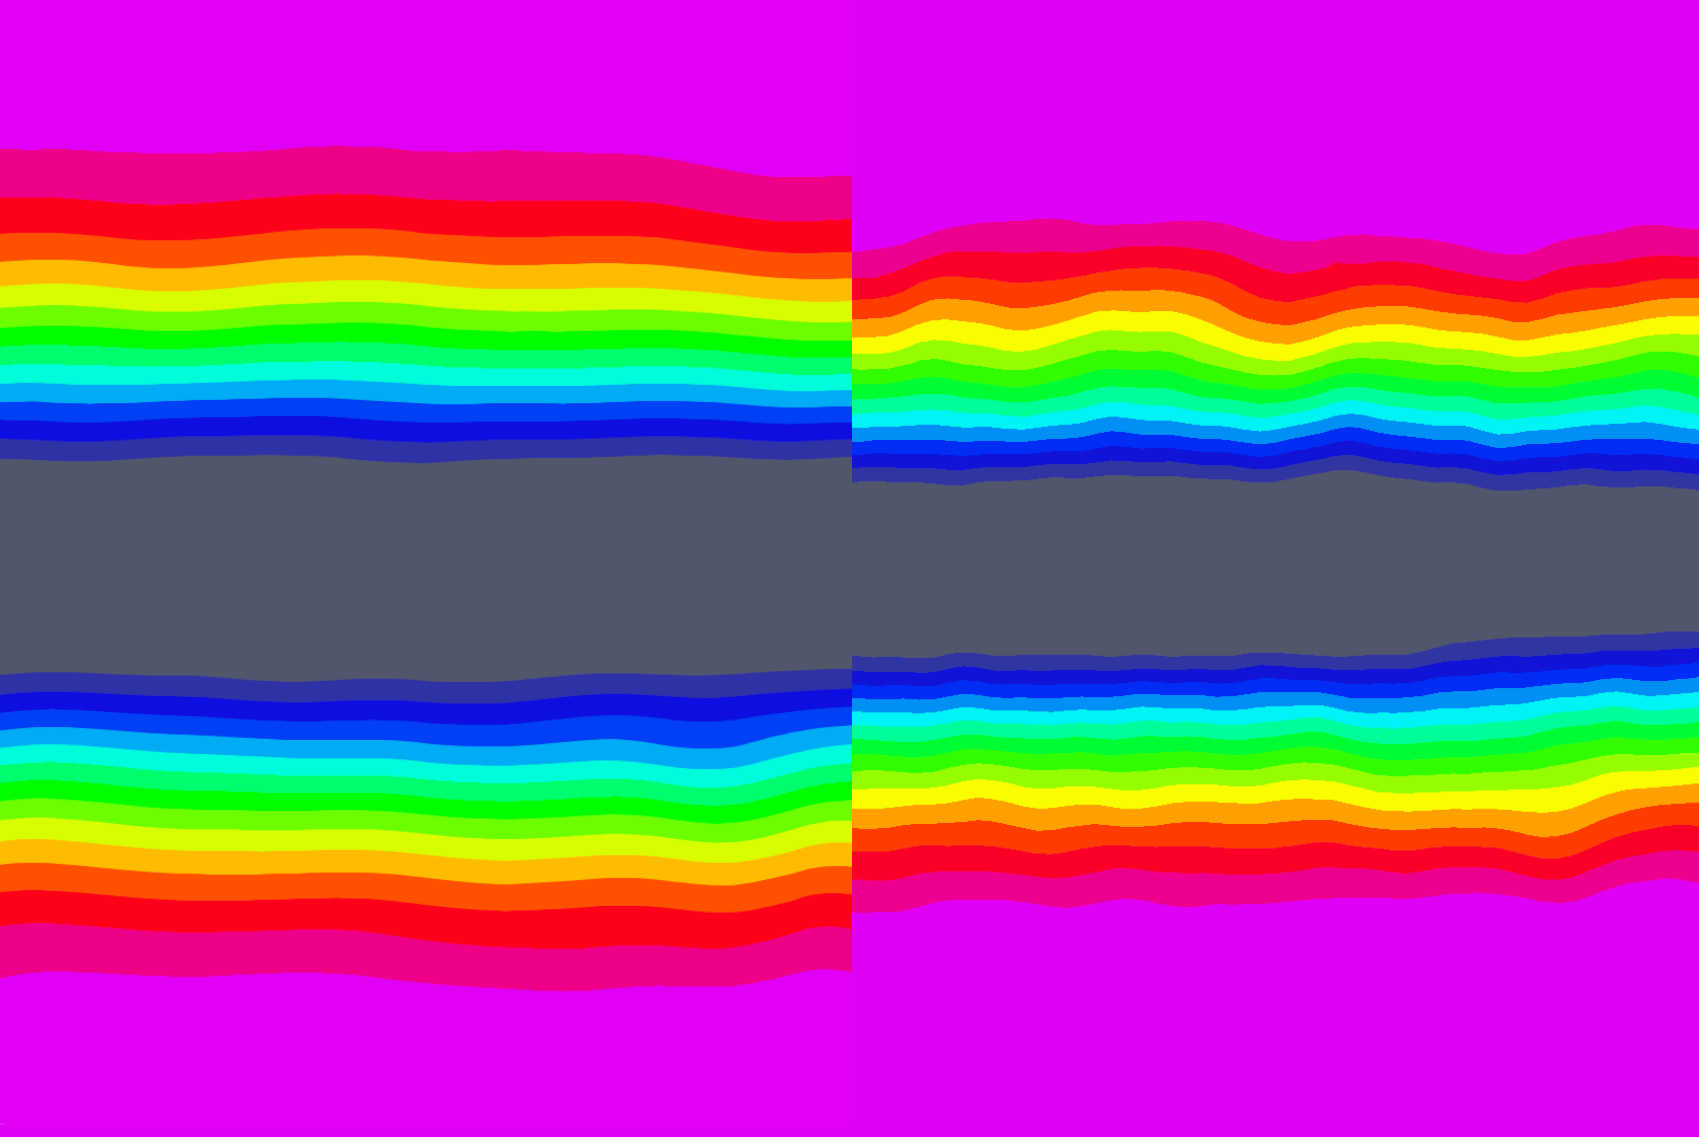
\includegraphics[trim = 0px 0px 0px 0px,clip,width = 0.39\textwidth]{\myImages/res/uXMeanCompPOM2.png}}
	\begin{axis}[
		name = plot1,
		xlabel={$z_r$ [--]},
		ylabel={$y_r$ [--]},
		font = \scriptsize,
		xtick distance=1,ytick distance=1,
		width=\wd\mygraphic,
		height=\ht\mygraphic, %height= 5/3*0.5
		enlargelimits=false,
		scale only axis=true,
		tick align=outside,
		ytick pos=left,
		xtick pos=bottom,
		y label style = {at={(axis cs:-3.6,0)}},
		x label style = {at={(axis cs:0,-2.7)}},
		line width = 1.7pt]
		\addplot graphics[xmin=-3, xmax=3, ymin=-2, ymax=2,includegraphics={trim = 0px 0px 0px 0px,clip}] {\myImages/res/uXMeanCompPOM2.png};
		% \fill [white] (axis cs:0.001,-1.997) rectangle (axis cs:0.5,1.997);
		% \fill [black!70](axis cs:0,0) circle [radius=0.5];
		% \draw [black,dashdotted,line width = 1.0pt] (axis cs:-2,0) -- (axis cs:2,0);
		\draw [black!70,dashed,line width = 1.0pt] (axis cs:0,2) -- (axis cs:0,-2);
		\node [white] at (axis cs:0.2,1.7) {\scriptsize{$\zeta$}};
		\node [white] at (axis cs:-2.55,1.75) {\scriptsize{PIV}};
		\node [white] at (axis cs:2.55,1.75) {\scriptsize{CFD}};
	\end{axis}
	\node [name = osaUx,anchor = south east,at={(plot1.north east)},yshift=0.07cm] {
\includegraphics[width=0.26\textwidth]{\myImages/res/U_x_scale2.png}};
	\node [name = ux, anchor = east,at={(osaUx.north west)},yshift=-0.1cm,xshift=-0.1cm] {\scriptsize{$u/u_{\mathrm{in}}$ [--]}};
	\node [name = psi0, anchor = south,at={(osaUx.north)},yshift=-0.2cm,xshift=-1.6cm] {\scriptsize{\ 0.7}};
	\node [name = psi0, anchor = west,at={(psi0.east)},xshift=0.45cm] {\scriptsize{0.8}};
	\node [name = psi0, anchor = west,at={(psi0.east)},xshift=0.45cm] {\scriptsize{0.9}};
	\node [name = psi0, anchor = west,at={(psi0.east)},xshift=0.45cm] {\scriptsize{1.0}};
	% \node [name = psi0, anchor = west,at={(psi0.east)},xshift=-0.11cm] {\scriptsize{0.98}};
	% \node [name = psi0, anchor = west,at={(psi0.east)},xshift=-0.14cm] {\scriptsize{1.02}};

	\savebox\mygraphic{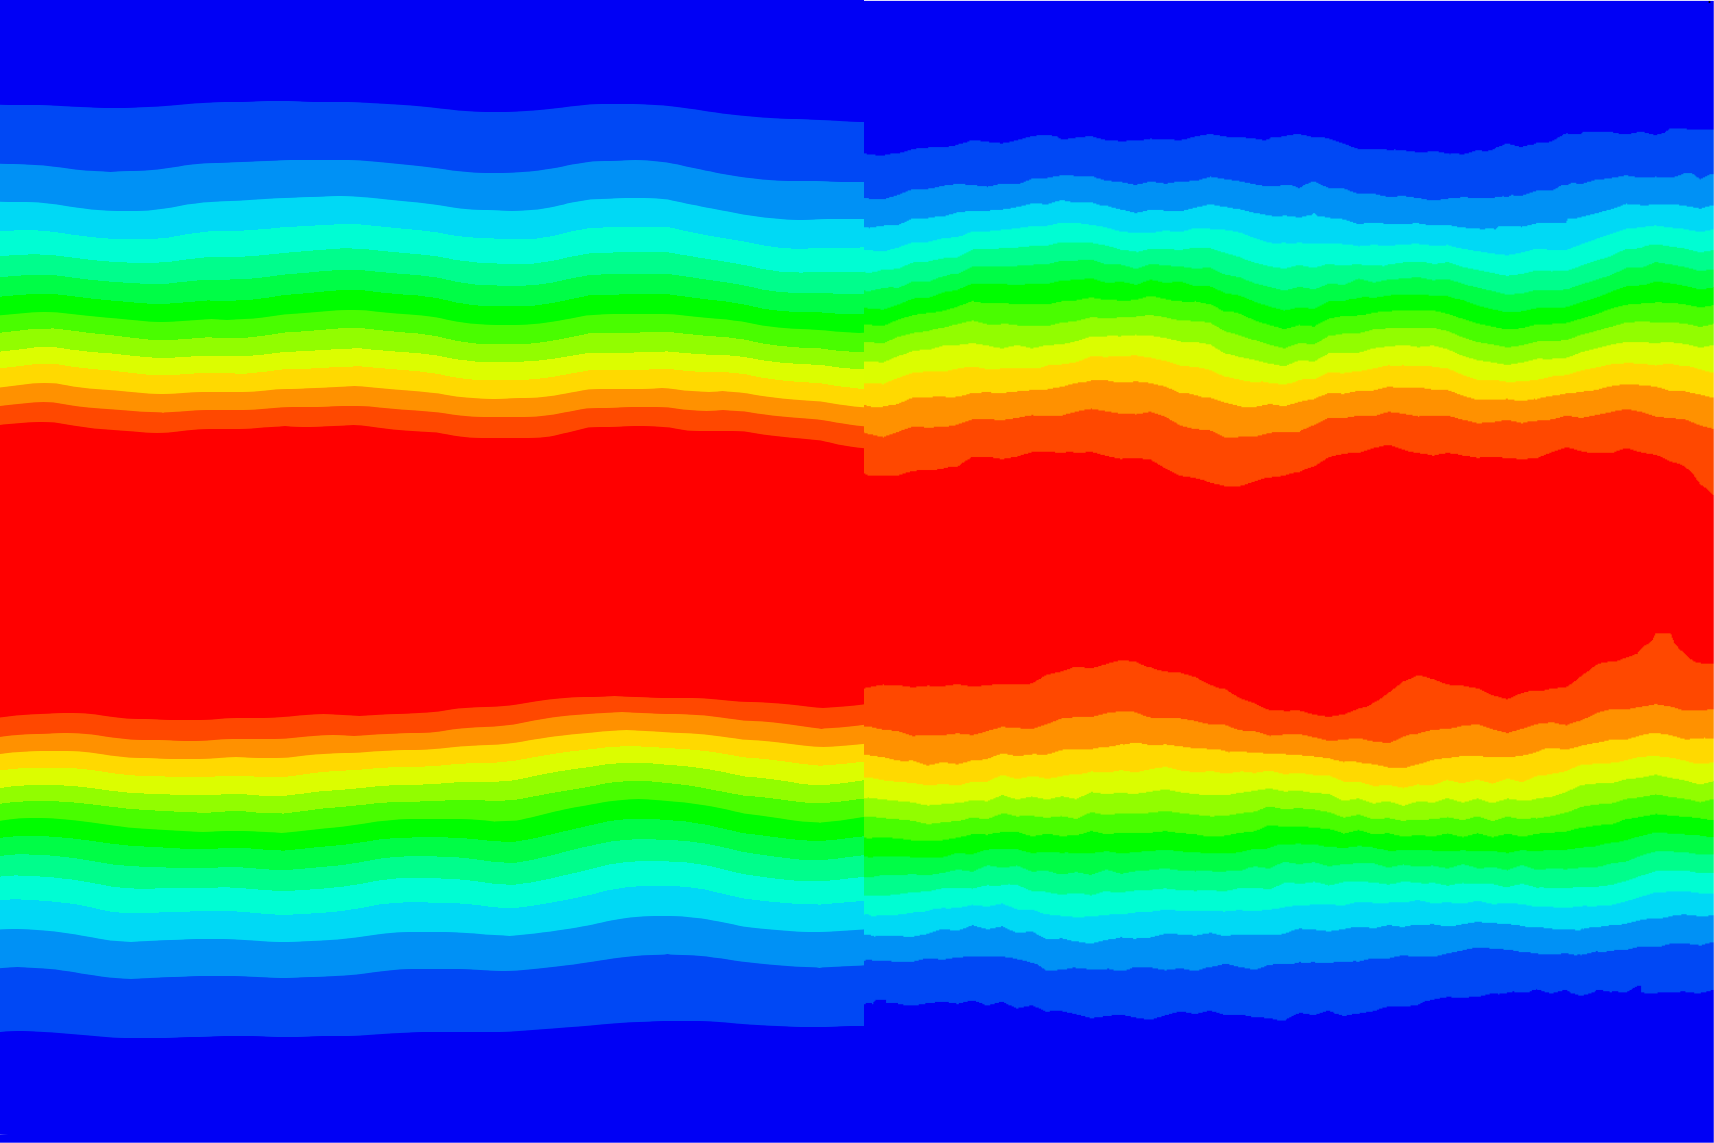
\includegraphics[trim = 0px 0px 0px 0px,clip,width = 0.39\textwidth]{\myImages/res/kMeanCompPOM2.png}}
	\begin{axis}[
		name = plot2,
		anchor = west,
		at = {(plot1.east)},
		xshift = 0.4cm,
		xlabel={$z_r$ [--]},
		ylabel={$y_r$ [--]},
		x label style = {at={(axis cs:0,-2.7)}},
		y label style = {at={(axis cs:3.5,0)}},
		font = \scriptsize,
		xtick distance=1,ytick distance=1,
		width=\wd\mygraphic,
		height=\ht\mygraphic, %height= 5/3*0.5
		enlargelimits=false,
		scale only axis=true,
		tick align=outside,
		ytick pos=right,
		xtick pos=bottom,
		line width = 1.7pt]
		\addplot graphics[xmin=-3, xmax=3, ymin=-2, ymax=2,includegraphics={trim = 0px 0px 0px 0px,clip}] {\myImages/res/kMeanCompPOM2.png};
		% \fill [white] (axis cs:0.001,-1.997) rectangle (axis cs:0.5,1.997);
		% \fill [black!70](axis cs:0,0) circle [radius=0.5];
		% \draw [black,dashdotted,line width = 1.0pt] (axis cs:-2,0) -- (axis cs:2,0);
		\draw [black!70,dashed,line width = 1.0pt] (axis cs:0,2) -- (axis cs:0,-2);
		\node [white] at (axis cs:0.2,1.7) {\scriptsize{$\zeta$}};
		\node [white] at (axis cs:-2.55,1.75) {\scriptsize{PIV}};
		\node [white] at (axis cs:2.55,1.75) {\scriptsize{CFD}};
	\end{axis}
	\node [name = osak,anchor = south east,at={(plot2.north east)},yshift=0.07cm,xshift=0.1cm] {
\includegraphics[width=0.26\textwidth]{\myImages/res/k_scale2.png}};
	\node [name = k, anchor = east,at={(osak.north west)},yshift=-0.1cm,xshift=-0.1cm] {\scriptsize{$k$ [--]}};
	\node [name = psi0, anchor = south,at={(osak.north)},yshift=-0.2cm,xshift=-1.49cm] {\scriptsize{0.00}};
	\node [name = psi0, anchor = west,at={(psi0.east)},xshift=0.03cm] {\scriptsize{0.04}};
	\node [name = psi0, anchor = west,at={(psi0.east)},xshift=0.03cm] {\scriptsize{0.08}};
	\node [name = psi0, anchor = west,at={(psi0.east)},xshift=0.03cm] {\scriptsize{0.12}};
	\node [name = psi0, anchor = west,at={(psi0.east)},xshift=0.03cm] {\scriptsize{0.15}};
	% \node [name = psi0, anchor = west,at={(psi0.east)},xshift=-0.2cm] {\scriptsize{0.28}};

	

\end{tikzpicture}